% Provenance (never printed): see sources/outline_sources.md (Year 1: the carbonate factory;
% reefs and platforms; pelagic oozes and the carbonate compensation depth; siliceous oozes;
% evaporite sequences). Exercise and problem values in the Book 3 scratch calculator
% calc/ch22.py; figure data from figdata/bachelor-1/evaporation.py and ccd_flank.py.
% Calcite, aragonite and dolomite are ch. 7's; the depth--age law ch. 13's; salinity Book 1's
% (g8); limestone Book 1's (g6, prose); the carbonate system and alkalinity the chemistry and
% biology books' (recalled, never defined). The subsidence of volcanic islands under reefs is
% the Year 2 volume's (oceanic islands); diagenesis (dolomitisation, chert, gypsum to
% anhydrite) is ch. 23's; upwelling ch. 29's.
\chapter{कार्बोनेट, सिलिसियस और वाष्पनिक तलछट}\label{ch:b1:chemical-biogenic-sediments}

इंग्लैंड और फ़्रांस के बीच की संकरी खाड़ी के दोनों ओर खड़ी सफ़ेद चॉक की चट्टानें सबसे साधारण चट्टानों जैसी लगती हैं। इलेक्ट्रॉन सूक्ष्मदर्शी के नीचे वे कैल्साइट की असंख्य छोटी पट्टियों से बनी निकलती हैं, जिन्हें उस समुद्र में तैरते एककोशिकीय शैवालों ने छोड़ा था जो कभी उस क्षेत्र को ढकता था। नाव से दिखने वाली एक \omterm{def:b1:chemical-biogenic-sediments:reef}{भित्ति} पैमाने के दूसरे छोर पर वही कहानी है: एक बनता हुआ चूना-पत्थर, जिसे प्रवाल और शैवाल पानी से कैल्शियम और कार्बोनेट लेकर पत्थर में बदलते हुए बनाते हैं। सभी तलछट बहकर नहीं आतीं; बहुत-सी वहीं बनती हैं, जीवित प्राणियों द्वारा, या स्वयं पानी द्वारा जब वह वाष्पित होता है। यह अध्याय तलछटों के तीन बड़े परिवारों का अनुसरण करता है --- कार्बोनेट, \omterm{def:b1:chemical-biogenic-sediments:ooze}{सिलिसियस ऊज़} और \omterm{def:b1:chemical-biogenic-sediments:evaporite}{वाष्पनिक निक्षेप} --- उस समुद्र की रसायन-विद्या से लेकर उन चट्टानों तक जिन्हें वे पीछे छोड़ते हैं।

\begin{recall}
चूना-पत्थर कैल्साइट से बनी एक अवसादी शैल है, प्रायः शंखों से, और तनु अम्ल में बुलबुले देती है (पुस्तक~1, कक्षा~6)। कैल्साइट और ऐरागोनाइट \ce{CaCO3} के दो \omterm{def:b1:rock-forming-minerals:polymorph}{बहुरूप} हैं, जिनके घनत्व \qty{2.71}{g.cm^{-3}} और \qty{2.93}{g.cm^{-3}} हैं, और डोलोमाइट \ce{CaMg(CO3)2}, जिसका घनत्व \qty{2.84}{g.cm^{-3}} है, कैल्शियम और मैग्नीशियम का कार्बोनेट है (\cref{ch:b1:rock-forming-minerals})। समुद्री जल की लवणता उसके एक किलोग्राम में घुले नमक का द्रव्यमान है (पुस्तक~1, कक्षा~8)। जल में कार्बन डाइऑक्साइड, हाइड्रोजन कार्बोनेट और कार्बोनेट आयन अम्ल-क्षार साम्यों से जुड़े हैं, और क्षारकता उन क्षारकों का माप है जो हाइड्रोजन आयनों को ग्रहण कर सकते हैं (रसायन-विज्ञान की पुस्तकें); महासागर का कार्बोनेट तंत्र कार्बन-चक्र का भाग है (जीव-विज्ञान की पुस्तकें)। समुद्र-तल आयु के साथ $d = d_r + C\sqrt t$ के अनुसार गहरा होता है (\cref{thm:b1:rifts-ridges-margins:depth-age})।
\end{recall}
% ledger: webmineral:polymorphs, hom:calcite, webmineral:others

\section{कार्बोनेट कारखाना}\label{sec:b1:chemical-biogenic-sediments:factory}

समुद्री जल में कैल्शियम और घुला अकार्बनिक कार्बन रहता है, अधिकतर हाइड्रोजन कार्बोनेट के रूप में। इन दोनों से कैल्शियम कार्बोनेट इन अभिक्रियाओं से बनता है:
\[
\ce{Ca^2+ + 2 HCO3- -> CaCO3 + CO2 + H2O}, \qquad
\ce{Ca^2+ + CO3^2- -> CaCO3},
\]
पहली अभिक्रिया में बने हर कार्बोनेट के साथ एक अणु कार्बन डाइऑक्साइड निकलता है। उष्णकटिबंधीय उष्ण सतही जल कैल्शियम कार्बोनेट से अतिसंतृप्त है, फिर भी वह शायद ही स्वयं अवक्षेपित होता है: लगभग सब कुछ जीवित प्राणी बनाते हैं, जो अपने शंख और कंकाल बनाने की ऊर्जा चुकाते हैं और उस \omterm{def:b1:rock-forming-minerals:mineral}{खनिज} को नियंत्रित करते हैं जिसका वे उपयोग करते हैं। प्रवाल और हरे शैवाल ऐरागोनाइट बनाते हैं; लाल शैवाल और अनेक फ़ोरामिनिफ़ेरा कैल्साइट बनाते हैं, जिसका कुछ भाग मैग्नीशियम से समृद्ध होता है; मोलस्का इनमें से एक या दोनों का उपयोग करते हैं।

\begin{definition}[कार्बोनेट कारखाना]\label{def:b1:chemical-biogenic-sediments:factory}
किसी समुद्र का \emph{कार्बोनेट कारखाना}\index{कार्बोनेट कारखाना} वे जीव और प्रक्रियाएँ हैं जो कैल्शियम कार्बोनेट तलछट वहीं बनाती हैं जहाँ वह पाई जाती है, न कि उसे कहीं और से लाया जाता है। उसके उत्पाद हैं कंकाल-कण (साबुत या टूटे शंख और कंकाल), कार्बोनेट कीचड़, लेपित कण और भित्तियों के कठोर ढाँचे।
\end{definition}

सबसे समृद्ध कारखाना गर्म, स्वच्छ, उथले और धूप वाले पानी में काम करता है, नदियों के कीचड़ से दूर, जो उत्पादकों को दबा देता और प्रकाश को धुँधला कर देता जिसकी शैवालों को ज़रूरत है। उसका तलछट समुद्र-तल स्वयं बनाता है: प्रवाल और शैवाल का मलबा, तल पर रहने वाले मोलस्का के शंख और एककोशिकीय फ़ोरामिनिफ़ेरा के खोल, और हरे शैवालों द्वारा छोड़ी गई ऐरागोनाइट की सुइयाँ, जो चूने के कीचड़ के रूप में बैठ जाती हैं। जहाँ पानी विक्षुब्ध और अतिसंतृप्त है, वहाँ लहरों और ज्वार से लुढ़कते कण एक केंद्रक के चारों ओर, जो बालू का एक कण या शंख का टुकड़ा हो सकता है, कार्बोनेट की परतें उगाते हैं और गोल \omterm{def:b1:chemical-biogenic-sediments:reef}{ऊइड} बन जाते हैं (\cref{def:b1:chemical-biogenic-sediments:reef})। एक दूसरा कारखाना खुले समुद्र में काम करता है, किसी तट से दूर: धूप वाली सतही परत में रहने वाले प्लवक छोटे कैल्साइट कवच और पट्टियाँ बनाते हैं जो गहरे समुद्र-तल पर बरसती हैं (\cref{sec:b1:chemical-biogenic-sediments:oozes})।
% ledger: og:carbonates

कारखाना कितनी तेज़ी से बनाता है, यह उसके कार्बोनेट बजट से मापा जाता है: एक वर्ग मीटर पर हर वर्ष उत्पादित और अपनी जगह रखा गया कार्बोनेट का द्रव्यमान, छेद करने वाले जीवों, चरने वालों और लहरों से होने वाली हानियों के बाद। वह द्रव्यमान-संतुलन से ऊर्ध्वाधर वृद्धि की दर में बदल जाता है।

\begin{proposition}[कार्बोनेट बजट से संचयन]\label{prop:b1:chemical-biogenic-sediments:accretion}
मान लीजिए एक समुद्र-तल प्रति इकाई क्षेत्रफल और प्रति इकाई समय में कैल्शियम कार्बोनेट का शुद्ध द्रव्यमान $G$ अपनी जगह रखता है, एक ऐसे निक्षेप के रूप में जिसके ठोस कणों का घनत्व $\rho_s$ है और जिसकी छिद्रता, यानी उसके आयतन का वह भाग जो छिद्र घेरते हैं, $\phi$ है। तब तल इस दर से ऊपर उठता है
\[
a = \frac{G}{\rho_s\,(1-\phi)}.
\]
\end{proposition}

\begin{proof}
पूरे समय $\mathrm dt$ में एक इकाई क्षेत्रफल पर कार्बोनेट का ठोस द्रव्यमान $G\,\mathrm dt$ आता है, जो कणों के आयतन $G\,\mathrm dt/\rho_s$ को भरता है। ये कण नई परत का भाग $1-\phi$ बनाते हैं, जिसकी मोटाई इसलिए $G\,\mathrm dt/(\rho_s(1-\phi))$ है। $\mathrm dt$ से भाग देने पर $a$ मिलता है।
\end{proof}

गुणनफल $\rho_s(1-\phi)$ निक्षेप का शुष्क थोक घनत्व है। चागोस द्वीपसमूह के हिंद महासागर के प्रवालों पर 2015 में मापी गई 28 भित्तियों का औसत बजट प्रति वर्ग मीटर और प्रति वर्ष \qty{3.7}{kg} \ce{CaCO3} था, और जिन भित्तियों पर शाखादार \emph{एक्रोपोरा} प्रवालों का प्रभुत्व था, उनका \qty{8.4}{kg} था, जो लगभग \qty{4.2}{mm} प्रति वर्ष बढ़ती थीं; संचयन के सूत्र के साथ ये दो संख्याएँ मिलकर \qty{2000}{kg.m^{-3}} का शुष्क थोक घनत्व बताती हैं, यानी एक भित्ति-ढाँचा जिसका लगभग एक-तिहाई भाग रिक्त स्थान है (\cref{exo:b1:chemical-biogenic-sediments:3})। उन्हीं भित्तियों ने 1998 की ऊष्मन घटना में अपने प्रवालों का नौ-दसवाँ भाग से अधिक खो दिया था, और उनके बजट दिखाते हैं कि \omterm{def:b1:chemical-biogenic-sediments:reef}{भित्ति} कितनी तेज़ी से पुनर्निर्माण कर सकती है।
% ledger: perry:chagos

\section{भित्तियाँ और मंच}\label{sec:b1:chemical-biogenic-sediments:reefs}

जहाँ कारखाना एक कठोर ढाँचा बनाता है, वह लहरों के सामने समुद्र-तल से ऊपर खड़ा हो सकता है।

\begin{definition}[भित्ति, कार्बोनेट मंच, ऊइड]\label{def:b1:chemical-biogenic-sediments:reef}
एक \emph{भित्ति}\index{भित्ति} एक कार्बोनेट उभार है जिसका ढाँचा, प्रवाल, शैवाल या अन्य जीव, अपनी जगह उगकर और एक-दूसरे से बँधकर और सीमेंटित होकर, आसपास के समुद्र-तल से ऊपर उठता है और लहरों का प्रतिरोध करता है। एक \emph{कार्बोनेट मंच}\index{कार्बोनेट मंच} उथले पानी के कार्बोनेट की एक मोटी राशि है जिसका सपाट शीर्ष समुद्र-स्तर के निकट है और जो गहरे पानी की ओर एक ढलान से घिरा होता है। एक \emph{ऊइड}\index{ऊइड} बालू के आकार का गोल कण है, जो कार्बोनेट की संकेंद्रित परतों से बना है, जो हिलते पानी में लुढ़कते समय एक केंद्रक के चारों ओर उगी हैं; ऊइडों से बनी चट्टान ऊलाइट है।
\end{definition}
% ledger: og:carbonates

समुद्री प्रवालों की तीन किस्में हैं, जिनके नाम उन नाविकों ने रखे जिन्होंने उनका मानचित्र बनाया, बहुत पहले कि कोई उनके आर-पार ड्रिल करता। एक \emph{तटीय} \omterm{def:b1:chemical-biogenic-sediments:reef}{भित्ति} किसी द्वीप या महाद्वीप के तट से जुड़ी होती है। एक \emph{अवरोधक} \omterm{def:b1:chemical-biogenic-sediments:reef}{भित्ति} भूमि से एक लैगून द्वारा अलग होती है, जो चौड़ा हो सकता है और दसियों मीटर गहरा; उत्तर-पूर्वी ऑस्ट्रेलिया की अवरोधक \omterm{def:b1:chemical-biogenic-sediments:reef}{भित्ति}, जगह-जगह टूटी हुई, लगभग एक हज़ार मील तक चलती है और 10 से 25 फ़ैदम गहरे एक समुद्र को घेरती है, यानी लगभग \qty{18}{m} से \qty{46}{m}। एक \emph{एटॉल} \omterm{def:b1:chemical-biogenic-sediments:reef}{भित्ति} का एक वलय है, जिसके ऊपर निचले प्रवाल-रेत के द्वीप हैं, और जिसके भीतर एक लैगून है जिसमें कोई भूमि नहीं।

\begin{omfigure}
\begin{tikzpicture}[font=\footnotesize, scale=0.72]
% three reef types in cross-section (schematic): a volcanic cone y = 2 - s - 0.75|x - 4|
% subsided by s (0, 0.8, 1.6), sea level at y = 1; the reef grows up from its first
% position, the foot of the fringing reef at (2, 0.5) moving down with the cone
\foreach \s/\yo/\lab/\name in {0/0/a/तटीय भित्ति, 0.8/-3.8/b/अवरोधक भित्ति, 1.6/-7.6/c/एटॉल} {
  \begin{scope}[yshift=\yo cm]
    \begin{scope}
      \clip (0,-1.3) rectangle (8,2.3);
      \fill[omSea] (0,-1.3) rectangle (8,1.0);
      \draw[lith basalt] (-1,2-\s-3.75) -- (4,2-\s) -- (9,2-\s-3.75) -- cycle;
    \end{scope}
    \draw[omSea!60!black] (0,1.0) -- (8,1.0);
    \node[anchor=west, font=\scriptsize] at (8.05,1.0) {समुद्र-स्तर};
    \node[anchor=west] at (0,2.05) {(\lab) \name};
    \draw[black!70] (1.05,1.55) node[anchor=east, font=\scriptsize] {भित्ति} -- (2.2,1.02);
  \end{scope}
}
% (a) fringing reef: wedges against the shore
\fill[lith reef limestone, draw=black!70] (2.0,0.5) -- (2.15,1.0) -- (2.667,1.0) -- cycle;
\fill[lith reef limestone, draw=black!70] (6.0,0.5) -- (5.85,1.0) -- (5.333,1.0) -- cycle;
\node[anchor=west, font=\scriptsize] at (4.9,1.75) {ज्वालामुखी द्वीप};
% (b) barrier reef: the cone has sunk by 0.8, the reef has grown up, a lagoon opens
\begin{scope}[yshift=-3.8cm]
  \fill[lith reef limestone, draw=black!70] (2.0,-0.3) -- (2.15,1.0) -- (2.6,1.0) -- (2.55,0.1125) -- cycle;
  \fill[lith reef limestone, draw=black!70] (6.0,-0.3) -- (5.85,1.0) -- (5.4,1.0) -- (5.45,0.1125) -- cycle;
  \draw[black!70] (3.2,0.85) -- (3.45,1.55) node[anchor=south west, font=\scriptsize, inner sep=1pt] {लैगून};
\end{scope}
% (c) atoll: the cone has sunk by 1.6 and is drowned; the reef ring encloses a lagoon
\begin{scope}[yshift=-7.6cm]
  \fill[lith limestone, draw=black!50] (2.55,-0.6875) -- (2.55,0.55) -- (5.45,0.55) -- (5.45,-0.6875) -- (4,0.4) -- cycle;
  \fill[lith reef limestone, draw=black!70] (2.0,-1.1) -- (2.15,1.0) -- (2.6,1.0) -- (2.55,-0.6875) -- cycle;
  \fill[lith reef limestone, draw=black!70] (6.0,-1.1) -- (5.85,1.0) -- (5.4,1.0) -- (5.45,-0.6875) -- cycle;
  \node[font=\scriptsize] at (4,0.78) {लैगून};
  \node[font=\scriptsize, fill=omLithLime, inner sep=1pt] at (4,0.05) {लैगून तलछट};
\end{scope}
% photograph
\node[anchor=north west, inner sep=0] at (10.75,2.3) {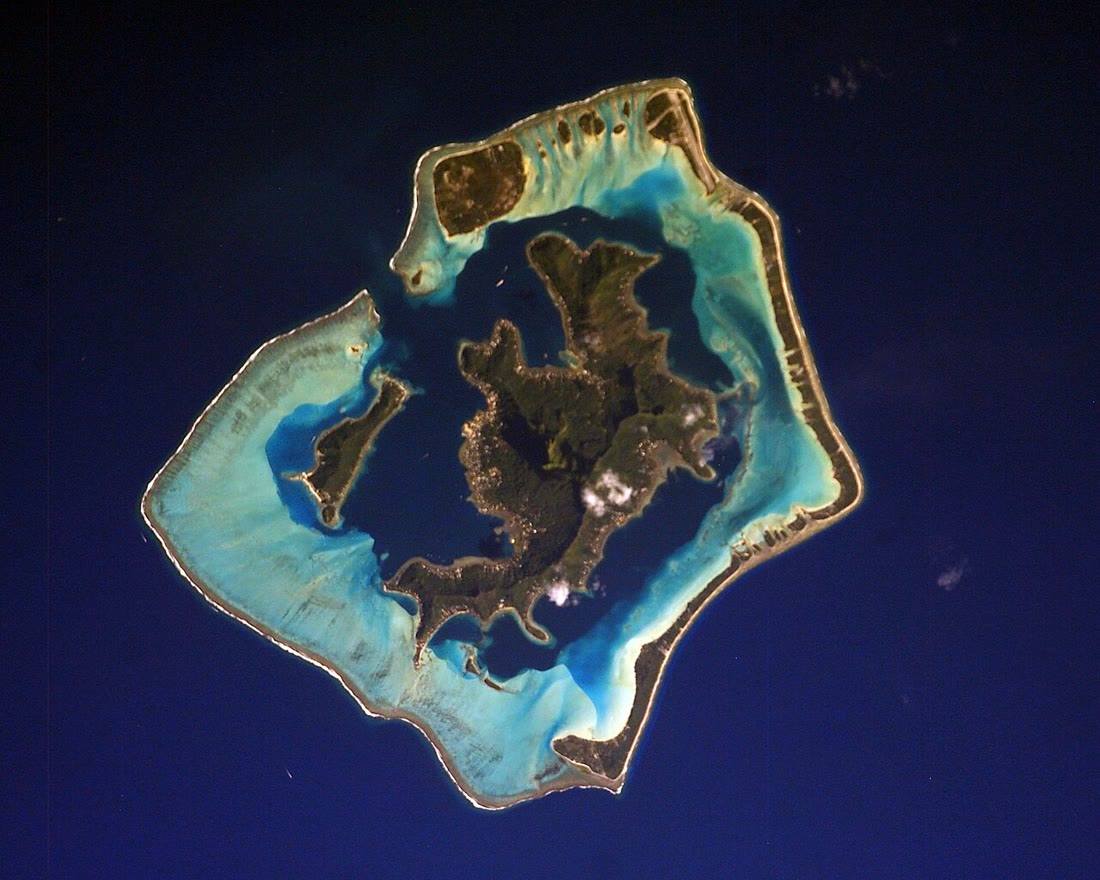
\includegraphics[height=6.9cm]{images/book3/b1-bora-bora.jpg}};
\end{tikzpicture}

{\small बाईं ओर: समुद्री प्रवालों की तीन किस्में अनुप्रस्थ काट में (योजनाबद्ध, ऊर्ध्वाधर पैमाना बहुत बढ़ाकर), डार्विन की व्याख्या के अनुसार बनी: (a)~एक ज्वालामुखी द्वीप से सटी एक तटीय \omterm{def:b1:chemical-biogenic-sediments:reef}{भित्ति}; (b)~द्वीप धँस गया है और \omterm{def:b1:chemical-biogenic-sediments:reef}{भित्ति}, ऊपर उगते हुए, एक लैगून द्वारा तट से अलग होकर अवरोधक बन गई है; (c)~द्वीप दृष्टि से ओझल होकर धँस गया है और \omterm{def:b1:chemical-biogenic-sediments:reef}{भित्ति} एक लैगून के चारों ओर एक एटॉल है, जिसकी तली कार्बोनेट तलछट से ढकी है। दाहिनी ओर: बोरा बोरा, एक ज्वालामुखी द्वीप, जो एक अवरोधक \omterm{def:b1:chemical-biogenic-sediments:reef}{भित्ति} से घिरे लैगून में है और उस पर निचले द्वीप हैं; अंतरिक्ष यात्री ने 19 मार्च 2003 को अंतरराष्ट्रीय अंतरिक्ष स्टेशन से इसका फ़ोटो लिया (फ़ोटो: NASA, सार्वजनिक डोमेन, विकिमीडिया कॉमन्स के माध्यम से)।}
\label{fig:b1:chemical-biogenic-sediments:reefs}
\end{omfigure}
% ledger: darwin:reefs, commons:bora-bora

\begin{history}[धँसती नींव पर भित्तियाँ, 1837--1842]
\emph{बीगल} की यात्रा के दौरान चार्ल्स डार्विन प्रशांत और हिंद महासागरों की भित्तियों के बीच घूमे। उन्होंने एक तथ्य से तर्क किया: प्रवाल-भित्ति बनाने वाले प्रवाल, उन्होंने निष्कर्ष निकाला, सामान्यतः 20 से 30 फ़ैदम के बीच की गहराई से गहरे नहीं पनपते, यानी लगभग 37 से \qty{55}{m} तक। फिर भी अवरोधक भित्तियाँ और एटॉल उस सीमा से कहीं नीचे के गहरे पानी से उठते हैं। उनकी नींव, उन्होंने तर्क दिया, अवश्य धँसी होगी, इतनी धीरे कि प्रवाल ऊपर बढ़कर अपने शीर्ष सतह पर रख सकें: ज्वालामुखी द्वीप से सटी \omterm{def:b1:chemical-biogenic-sediments:reef}{भित्ति}, द्वीप के भीतर धँसने पर, अवरोधक बन जाती है, और द्वीप लुप्त होने पर एटॉल। उन्होंने अपना सिद्धांत 31 मई 1837 को लंदन की भूवैज्ञानिक सोसाइटी के समक्ष पढ़ा और 1842 में \emph{प्रवाल-भित्तियों की संरचना और वितरण} नाम से प्रकाशित किया, जिसमें विश्व की सभी भित्तियों का एक मानचित्र था जो तीन किस्मों में छाँटी गई थीं। महासागरीय द्वीप क्यों और कितना धँसते हैं, यह उस प्लेट के ठंडे होने का विषय है जिसके ऊपर वे हैं, जिसे पुस्तक~4 में लिया गया है।
\end{history}
% ledger: darwin:reefs

एक \omterm{def:b1:chemical-biogenic-sediments:reef}{भित्ति} तभी बचती है जब उसका शीर्ष उथले पानी में रहे, जहाँ उसके निर्माता जीते हैं। समुद्र-स्तर बदलता है, और नींव धँस सकती है; मायने यह रखता है कि दोनों का योग, यानी समुद्र-स्तर की सापेक्ष वृद्धि, क्या है।

\begin{proposition}[ऊपर उठो या डूबो]\label{prop:b1:chemical-biogenic-sediments:keep-up}
मान लीजिए \omterm{def:b1:chemical-biogenic-sediments:reef}{भित्ति} का शीर्ष समुद्र-स्तर से नीचे $D_0$ गहराई पर है और वह दर $a$ से ऊपर बढ़ता है, जबकि सापेक्ष समुद्र-स्तर दर $r$ से बढ़ता है, दोनों स्थिर। तब समय $t$ के बाद \omterm{def:b1:chemical-biogenic-sediments:reef}{भित्ति} के ऊपर पानी की गहराई
\[
D(t) = D_0 + (r - a)\,t .
\]
यदि $a \ge r$, तो \omterm{def:b1:chemical-biogenic-sediments:reef}{भित्ति} समुद्र के साथ बनी रहती है (जब $a > r$ तो उसका शीर्ष सतह तक पहुँचता है, और उसके बाद वह केवल पार्श्वतः बढ़ सकती है); यदि $a < r$, तो वह पिछड़ती है, और यदि उसके निर्माता $D_{\max}$ से गहरे नहीं जी सकते, तो समय $(D_{\max} - D_0)/(r - a)$ के बाद वह डूब जाती है।
\end{proposition}

\begin{proof}
\omterm{def:b1:chemical-biogenic-sediments:reef}{भित्ति} के शीर्ष की ऊँचाई $h_0 + a t$ है और समुद्र की सतह $s_0 + r t$ है, इसलिए शीर्ष के ऊपर पानी की गहराई $D = (s_0 - h_0) + (r - a)t = D_0 + (r-a)t$ है। जब $a > r$, तो $D$ समय $t = D_0/(a-r)$ पर शून्य होता है और \omterm{def:b1:chemical-biogenic-sediments:reef}{भित्ति} समुद्र के ऊपर नहीं उग सकती। जब
$a < r$, $D$ रैखिक रूप से बढ़ता है और $D_{\max}$ तक पहुँचता है जब $(r-a)t = D_{\max} -
D_0$।
\end{proof}

जिस \omterm{def:b1:chemical-biogenic-sediments:reef}{भित्ति} का शीर्ष डूब चुका है, वह तुरंत मरती नहीं, पर प्रकाश धुँधला पड़ता है, निर्माता बदल जाते हैं और कारखाना धीमा हो जाता है, इसलिए जो \omterm{def:b1:chemical-biogenic-sediments:reef}{भित्ति} पिछड़ने लगती है वह और पिछड़ती जाती है: डूबी हुई भित्तियाँ और मंच, जिनके ऊपर गहरे पानी के तलछट जमे हैं, कई महासागरीय द्वीपों की ढलानों पर और शैल-अभिलेख में मिलते हैं।

लाखों वर्षों में कारखाने \omterm{def:b1:chemical-biogenic-sediments:reef}{कार्बोनेट मंच} बनाते हैं, उथले पानी के कार्बोनेट की मोटी राशियाँ जो उनकी नींव के धँसने के साथ बढ़ती हैं। दो आकार बार-बार मिलते हैं (नीचे का चित्र देखिए)। एक \emph{किनारेदार शेल्फ़} का सपाट शीर्ष होता है, जो अपने किनारे पर भित्तियों और ऊइड-टीलों के एक घेरे से संरक्षित होता है, जो लहरों को तोड़ता है; उसके पीछे चूने के कीचड़ का शांत लैगून है, और सामने एक खड़ी ढलान, जहाँ घेरे से गिरे खंड और मलबा बेसिन तक जाते हैं। एक \emph{ढाल} बिना किसी विराम के तट से बेसिन तक बहुत धीरे ढलती है: जहाँ लहरें तल को हिलाती हैं वहाँ ऊइड-टीले और शंख-पट्टियाँ, फिर तूफ़ानों द्वारा बहाए गए शंख-मलबे के बिस्तर, फिर लहरों की पहुँच के नीचे चूने का कीचड़। किनारेदार शेल्फ़ मुख्यतः अपने घेरे से ऊपर और बाहर की ओर बढ़ता है, और ढाल अपनी तलछट-पट्टियों को समुद्र के उठने या गिरने के साथ तट की ओर या समुद्र की ओर खिसकाकर।

\begin{omfigure}
\begin{tikzpicture}[font=\footnotesize, >={Stealth[length=4pt]}]
% (a) rimmed shelf and (b) ramp, schematic cross-sections
\begin{scope}
  \fill[omSea] (0,0.2) rectangle (7.2,2.0);
  \fill[lith limestone, draw=black!60] (0,0) -- (0,1.55) -- (4.3,1.55) -- (4.5,1.75) -- (4.9,1.75) -- (5.1,1.5) -- (6.4,0.35) -- (7.2,0.3) -- (7.2,0) -- cycle;
  \fill[lith reef limestone, draw=black!70] (4.3,1.55) -- (4.5,1.75) -- (4.9,1.75) -- (5.1,1.5) -- (4.8,1.05) -- (4.3,1.05) -- cycle;
  \draw[omSea!60!black] (0,2.0) -- (7.2,2.0);
  \node at (2.1,1.78) {लैगून: चूने का कीचड़};
  \node[anchor=south, align=center, font=\scriptsize] at (4.7,2.05) {भित्ति-घेरा और\\ ऊइड-टीले};
  \node[anchor=west, font=\scriptsize] at (5.6,1.2) {ढलान: मलबा};
  \node[font=\scriptsize] at (6.75,0.75) {बेसिन};
  \node at (3.6,-0.35) {(a) किनारेदार शेल्फ़};
\end{scope}
\begin{scope}[xshift=8.0cm]
  \fill[omSea] (0,0.2) rectangle (7.2,2.0);
  \fill[lith limestone, draw=black!60] (0,0) -- (0,1.85) -- (7.2,0.55) -- (7.2,0) -- cycle;
  \draw[omSea!60!black] (0,2.0) -- (7.2,2.0);
  \draw[densely dashed, black!50] (0,1.6) -- (7.2,1.6) node[pos=1, anchor=south east, font=\scriptsize, inner sep=1pt] {साधारण मौसम की लहरें पहुँचती हैं};
  \draw[densely dashed, black!50] (0,1.0) -- (7.2,1.0) node[pos=1, anchor=south east, font=\scriptsize, inner sep=1pt] {तूफ़ानी लहरें पहुँचती हैं};
  \node[anchor=south, font=\scriptsize] at (0.9,2.05) {ऊइड-टीले};
  \node[anchor=south, font=\scriptsize] at (3.4,2.05) {तूफ़ानी शंख-बिस्तर};
  \node[anchor=south, font=\scriptsize] at (6.1,2.05) {चूने का कीचड़};
  \node at (3.6,-0.35) {(b) ढाल};
\end{scope}
\end{tikzpicture}

{\small दो आकार के \omterm{def:b1:chemical-biogenic-sediments:reef}{कार्बोनेट मंच} (योजनाबद्ध, ढलानें बहुत बढ़ाकर दिखाई गई हैं)। (a)~एक किनारेदार शेल्फ़: भित्तियों और ऊइड-टीलों का एक घेरा लहरों को तोड़ता है, उसके पीछे चूने के कीचड़ का शांत लैगून है, और घेरे से गिरा मलबा ढलान से नीचे बेसिन में जाता है। (b)~एक ढाल तट से बेसिन तक धीरे ढलता है, और उसके तलछट उस गहराई से छँटे हुए हैं जहाँ तक लहरें पहुँचती हैं।}
\label{fig:b1:chemical-biogenic-sediments:platforms}
\end{omfigure}

\section{पेलाजिक ऊज़ और कार्बोनेट क्षतिपूर्ति गहराई}\label{sec:b1:chemical-biogenic-sediments:oozes}

तट से दूर, समुद्र-तल महाद्वीपों से लगभग कुछ नहीं पाता, सिवाय सबसे बारीक हवा-बहाई धूल के। उस पर इसके बजाय जो गिरता है वह उन प्लवकों के कंकाल हैं जो किलोमीटरों ऊपर धूप वाले पानी में रहते थे: कोकोलिथोफ़ोर की कैल्साइट पट्टियाँ और फ़ोरामिनिफ़ेरा के शंख, डायटम के ओपल के फ़स्टूल और रेडियोलेरियनों के कंकाल (जिनका चित्र आगे दिया गया है)। कोकोलिथों की लंबी वर्षा समुद्र-तल पर वह मुख्य प्रक्रिया है जो चॉक और दुनिया के अधिकांश चूना-पत्थर को बनाती है।
% ledger: nasa:coccoliths-b3, og:carbonates

\begin{definition}[कैल्केरियस ऊज़, सिलिसियस ऊज़]\label{def:b1:chemical-biogenic-sediments:ooze}
ऊज़ एक बारीक-कणों वाला पेलाजिक तलछट है, जो खुले समुद्र में जमता है और मुख्यतः प्लवकों के कंकालों से बना होता है। यह एक \emph{कैल्केरियस ऊज़}\index{कैल्केरियस ऊज़} है जब कंकाल कैल्शियम कार्बोनेट के हों, मुख्यतः कोकोलिथ और फ़ोरामिनिफ़ेरा, और एक \emph{सिलिसियस ऊज़}\index{सिलिसियस ऊज़} है जब वे ओपल के हों, यानी जलयोजित अनाकार सिलिका, मुख्यतः डायटम और रेडियोलेरियन।
\end{definition}
% ledger: og:carbonates

\omterm{def:b1:chemical-biogenic-sediments:ooze}{कैल्केरियस ऊज़} समुद्र-तल के लगभग आधे भाग को ढकते हैं, पर केवल एक निश्चित गहराई तक: लगभग \qty{4500}{m} से नीचे वे लुप्त हो जाते हैं। कंकाल वहाँ गिरना बंद नहीं करते; वे घुल जाते हैं। गहरा समुद्र ठंडा है और दाब ऊँचा है, और कैल्साइट की विलेयता गहराई के साथ बढ़ती है, मुख्यतः दाब के कारण, जबकि पानी में कार्बोनेट आयन की सांद्रता सामान्यतः गहराई के साथ घटती है (इन साम्यों की रसायन-विद्या रसायन-विज्ञान की पुस्तकों से स्मरण की गई है)। एक निश्चित गहराई से नीचे गहरा पानी कैल्साइट के प्रति अल्पसंतृप्त है, और तल तक पहुँचने वाले कंकाल जितना गहरे पड़े हों उतनी तेज़ी से घुलते हैं।
% ledger: britannica:ccd, slotnick:ccd-definitions

\begin{omfigure}
\begin{tikzpicture}
\node[inner sep=0] (a) at (0,0) {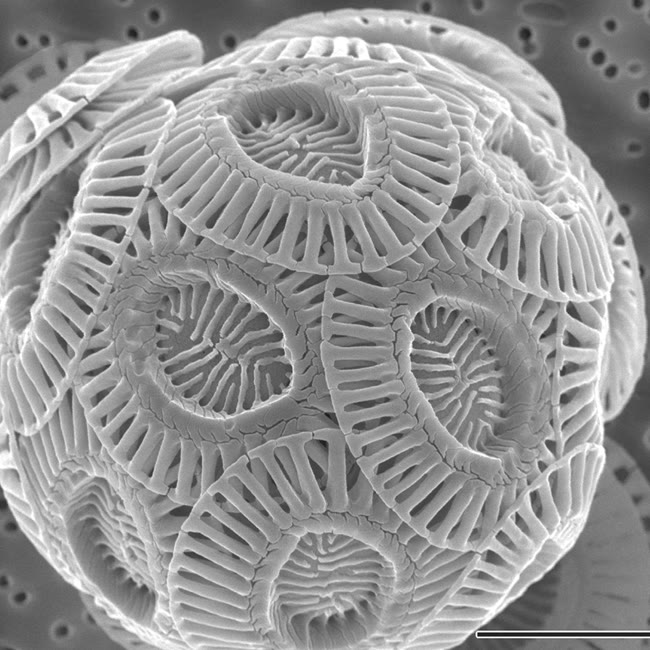
\includegraphics[height=4.3cm]{images/book3/b1-coccolithophore.jpg}};
\node[inner sep=0, anchor=west] (b) at ([xshift=0.25cm]a.east) {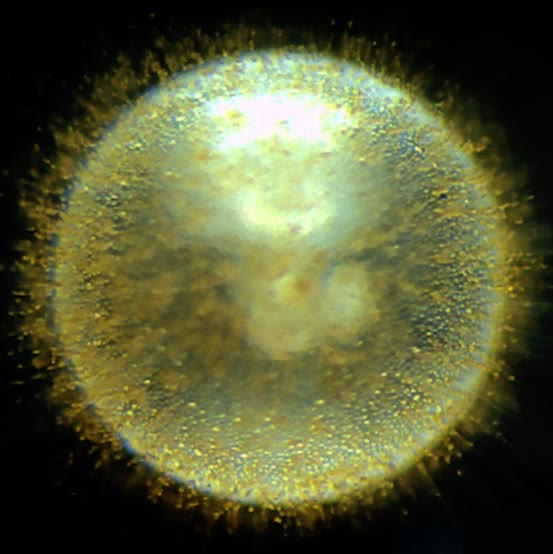
\includegraphics[height=4.3cm]{images/book3/b1-orbulina.jpg}};
\node[inner sep=0, anchor=west] (c) at ([xshift=0.25cm]b.east) {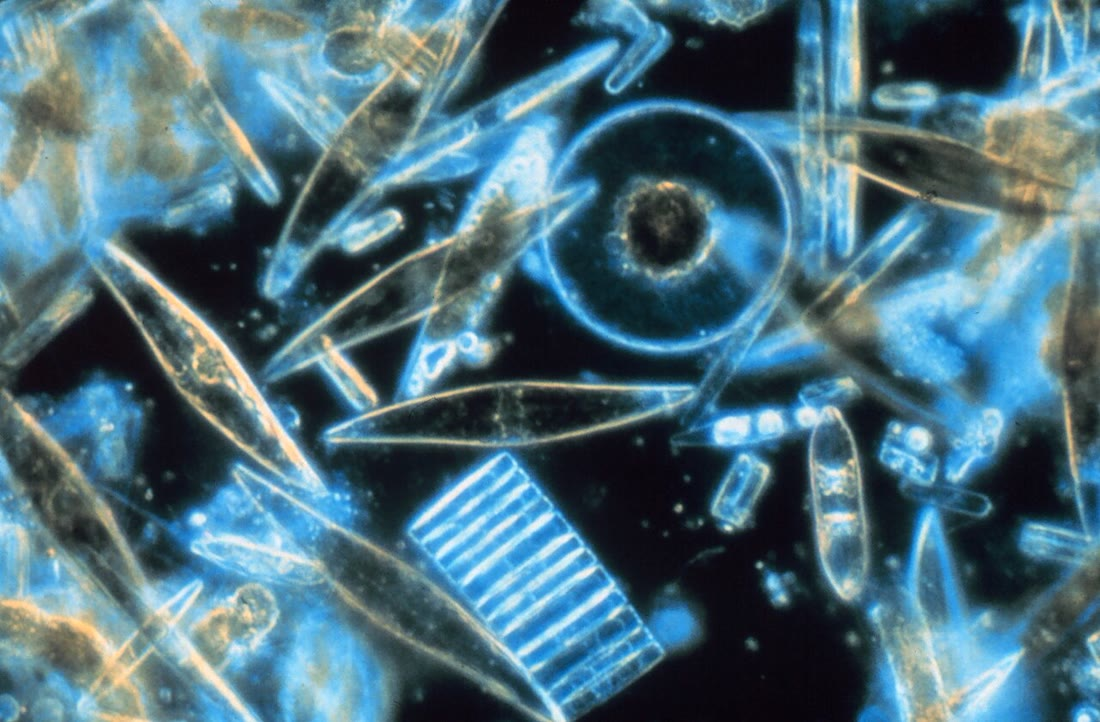
\includegraphics[height=4.3cm]{images/book3/b1-diatoms.jpg}};
\node[font=\footnotesize, anchor=north] at (a.south) {(a) एक कोकोलिथोफ़ोर};
\node[font=\footnotesize, anchor=north] at (b.south) {(b) एक फ़ोरामिनिफ़र};
\node[font=\footnotesize, anchor=north] at (c.south) {(c) डायटम};
\end{tikzpicture}

{\small जीवों का परिचय, जो ऊज़ बनाते हैं। (a)~एक \emph{एमिलियानिया हक्सलेई} कोशिका, जो अपनी कैल्साइट पट्टियों, यानी कोकोलिथों से ढकी है (स्कैनिंग इलेक्ट्रॉन सूक्ष्मदर्शी; फ़ोटो: Alison R.~Taylor, University of North Carolina Wilmington, CC~BY~2.5, विकिमीडिया कॉमन्स के माध्यम से)। (b)~एक जीवित प्लवकी फ़ोरामिनिफ़र, \emph{ऑर्बुलिना यूनिवर्सा}, जिसका कैल्साइट कवच काँटों से घिरा है (प्रकाश सूक्ष्मदर्शी; फ़ोटो: H.~Takagi और सहलेखक, 2019, CC~BY~4.0, विकिमीडिया कॉमन्स के माध्यम से)। (c)~समुद्री बर्फ़ से, मैकमर्डो साउंड, अंटार्कटिका, में जीवित डायटम, हर एक अपने ओपल के फ़स्टूल में (प्रकाश सूक्ष्मदर्शी; फ़ोटो: Gordon T.~Taylor, Stony Brook University, NOAA, सार्वजनिक डोमेन, विकिमीडिया कॉमन्स के माध्यम से)।}
\label{fig:b1:chemical-biogenic-sediments:plankton}
\end{omfigure}
% ledger: commons:ehux, commons:orbulina, commons:diatoms-noaa

\begin{definition}[लाइसोक्लाइन, कार्बोनेट क्षतिपूर्ति गहराई]\label{def:b1:chemical-biogenic-sediments:ccd}
\emph{लाइसोक्लाइन}\index{लाइसोक्लाइन} वह समुद्री गहराई है जिसके नीचे समुद्र-तल पर कैल्साइट का घुलना तलछट में पहली बार दिखने लगता है और उसकी दर तेज़ी से बढ़ती है। \emph{कार्बोनेट क्षतिपूर्ति गहराई}\index{कार्बोनेट क्षतिपूर्ति गहराई} (CCD) वह गहराई है जिस पर कैल्साइट के घुलने की दर उस दर के बराबर होती है जिस पर कैल्साइट समुद्र-तल पर बरसता है; उसके नीचे कैल्शियम कार्बोनेट जमा नहीं होता। व्यवहार में उसे वहाँ रखा जाता है जहाँ सतही तलछट में कैल्शियम कार्बोनेट का भार \qty{10}{\%} से नीचे गिर जाता है।
\end{definition}
% ledger: slotnick:ccd-definitions

CCD आम तौर पर \omterm{def:b1:chemical-biogenic-sediments:ccd}{लाइसोक्लाइन} से सैकड़ों मीटर नीचे है। वह कोई स्थिर स्तर नहीं है: उसे आपूर्ति और घुलने के संतुलन से तय किया जाता है, इसलिए वह वहाँ गहरा होता है जहाँ प्लवक अधिक कार्बोनेट बनाते हैं और जहाँ गहरा पानी कम संक्षारक है। अटलांटिक में वह प्रशांत की तुलना में लगभग \qty{500}{m} गहरा है, जिसका कारण कार्बोनेट की अधिक आपूर्ति और धीमा घुलना दोनों हैं; पश्चिमी प्रशांत के भीतर ही वह उत्तर-पश्चिम में लगभग \qty{4000}{m} और मध्य प्रशांत में लगभग \qty{5100}{m} पर है। ऐरागोनाइट, जो कैल्साइट से अधिक विलेय है, और भी उथली गहराइयों पर घुल जाता है। भूवैज्ञानिक समय में आपूर्ति, उत्पादकता और घुलने में बदलावों ने CCD को \qty{2000}{m} से अधिक खिसकाया है।
% ledger: slotnick:ccd-definitions, britannica:ccd, zhang:ccd-west-pacific

\begin{method}[लाइसोक्लाइन और CCD का पता लगाना]\label{met:b1:chemical-biogenic-sediments:ccd}
\begin{enumerate}
  \item एक ही क्षेत्र में भिन्न गहराइयों वाले स्थानों से तलछट की ऊपरी कुछ सेंटीमीटर परत एकत्र कीजिए, इतनी दूर कि भूमि और ऊपर उठते जल से दूर रहें, ताकि मृत्तिका या ओपल से तनुकरण छोटा रहे।
  \item हर नमूने का \ce{CaCO3} भार-प्रतिशत मापिए और उसे जल की गहराई के विरुद्ध आलेखित कीजिए।
  \item \omterm{def:b1:chemical-biogenic-sediments:ccd}{लाइसोक्लाइन} वह गहराई है जहाँ मात्रा तीव्रता से गिरने लगती है, और जहाँ खोल घुलने के पहले चिह्न दिखाते हैं (टूटे, खुरचे हुए फ़ोरामिनिफ़ेरा)।
  \item CCD वह गहराई है जहाँ मात्रा \qty{10}{\%} तक गिरती है: दोनों ओर के दो नमूनों के बीच रैखिक अंतर्वेशन से उसे पढ़िए।
\end{enumerate}
\end{method}

समुद्र-तल के मध्य-महासागरीय कटक की ढलान पर, अक्ष के पास समुद्र-तल युवा और उथला होता है और आयु के साथ, जैसे-जैसे वह अक्ष से दूर जाता है, डूबता है। CCD के ऊपर जन्मा तल का एक टुकड़ा तब तक \omterm{def:b1:chemical-biogenic-sediments:ooze}{कैल्केरियस ऊज़} जमा करता है जब तक वह CCD के नीचे न डूब जाए; उसके बाद उसे वही मिलता है जो नहीं घुलता: ऊपर से हवा में जमी धूल, लोहे और मैंगनीज़ के ऑक्साइड, मछलियों के दाँत। यह धीमा, भूरा निक्षेप गहरे द्रोणियों की लाल मृत्तिका है।

\begin{proposition}[CCD पार करना]\label{prop:b1:chemical-biogenic-sediments:flank}
आयु $t$ के समुद्र-तल को गहराई $d(t) = d_r + C\sqrt t$ पर मान लीजिए
(\cref{thm:b1:rifts-ridges-margins:depth-age}), जिसमें कटक-अक्ष की गहराई $d_r$ है, जो एक स्थिर \omterm{def:b1:chemical-biogenic-sediments:ccd}{कार्बोनेट क्षतिपूर्ति गहराई} $z_c$ से उथली है। तब तल उस आयु पर CCD के नीचे से गुज़रता है
\[
t_c = \left(\frac{z_c - d_r}{C}\right)^2 ,
\]
और आयु $t > t_c$ वाला एक स्थान नीचे से ऊपर की ओर रखता है: ज्वालामुखी क्रस्ट, समय $t_c$ के दौरान जमा \omterm{def:b1:chemical-biogenic-sediments:ooze}{कैल्केरियस ऊज़}, और समय $t - t_c$ के दौरान जमी लाल मृत्तिका।
\end{proposition}

\begin{proof}
गहराई $d(t)$, $t$ के साथ बढ़ती है, और $d(t_c) = z_c$ से $C\sqrt{t_c} =
z_c - d_r$ मिलता है, अतः $t_c$। $t_c$ से पहले तल CCD के ऊपर रहता है, जहाँ कैल्साइट घुलने से तेज़ बरसता है और ऊज़ जमा होता है; $t_c$ के बाद वह नीचे रहता है, जहाँ कोई कार्बोनेट जमा नहीं होता और केवल अघुलनशील मृत्तिका जुड़ती है। ऊज़, जब मृत्तिका के नीचे दब जाता है, ऊपर के संक्षारक पानी से सुरक्षित हो जाता है, इसलिए परतों का क्रम समय के क्रम के अनुसार है।
\end{proof}

$d = 2500 + 350\sqrt t$ के साथ (मीटर में, $t$ दस लाख वर्षों में), \qty{4500}{m} पर रखा CCD आयु $(2000/350)^2 = \qty{32.7}{Myr}$ पर पार होता है; \qty{25}{mm} प्रति वर्ष की अर्ध-प्रसार दर पर यह अक्ष से \qty{816}{km} दूर है (नीचे का चित्र)। पुराने महासागर-तल में ड्रिल करने पर यही क्रम बार-बार मिलता है: बेसाल्ट, फिर \omterm{def:b1:chemical-biogenic-sediments:ooze}{कैल्केरियस ऊज़} या चॉक, फिर लाल मृत्तिका, तल की ढलान पर उतरने की यात्रा का अभिलेख। जहाँ प्लेट बाद में उच्च उत्पादकता की पेटी के नीचे, भूमध्य रेखा के पास, खिसक गई है, वहाँ मृत्तिका के ऊपर ऊज़ की नई परत जम सकती है; इसी से क्रोड प्लेटों की गति के साथ-साथ CCD की गहराई भी दर्ज करते हैं।
% ledger: parsons:plate-model

\begin{omfigure}
\begin{tikzpicture}[font=\footnotesize]
\begin{axis}[width=11cm, height=5.6cm, xmin=0, xmax=1750, ymin=2000, ymax=6200, y dir=reverse,
    xlabel={कटक-अक्ष से दूरी (km), अर्ध-प्रसार दर \qty{25}{mm.yr^{-1}}},
    ylabel={गहराई (m)}, ytick={2000,3000,...,6000},
    axis on top, clip=false]
  % sea water above the floor
  \addplot[fill=omSea, draw=none] table[x=x_km, y=depth] {figdata/out/bachelor-1-ccd_flank-profile.dat} -- (axis cs:1750,2000) -- (axis cs:0,2000) -- cycle;
  % floor: ooze-covered above the CCD, red clay below
  \addplot[very thick, draw=omLithLime!70!black, restrict x to domain=0:816.3] table[x=x_km, y=depth] {figdata/out/bachelor-1-ccd_flank-profile.dat};
  \addplot[very thick, draw=brown!70!black, restrict x to domain=816.3:1750] table[x=x_km, y=depth] {figdata/out/bachelor-1-ccd_flank-profile.dat};
  \draw[thick, omThm, densely dashed] (axis cs:0,4500) -- (axis cs:1750,4500) node[pos=0.99, anchor=north east, inner sep=1.5pt] {CCD, \qty{4500}{m}};
  \draw[black!60, dotted, thick] (axis cs:0,4050) -- (axis cs:1750,4050) node[pos=0.99, anchor=south east, inner sep=1.5pt] {लाइसोक्लाइन (योजनाबद्ध)};
  \fill[omThm] (axis cs:816.3,4500) circle[radius=2pt];
  \node[anchor=north east, align=right] at (axis cs:790,4620) {तल CCD को पार करता है\\ \qty{32.7}{Myr} पर, \qty{816}{km} दूर};
  \node[anchor=north, align=center, omLithLime!40!black] at (axis cs:520,2750) {कैल्केरियस ऊज़\\ जमा होता है};
  \node[anchor=north west, align=left, brown!60!black] at (axis cs:1000,5180) {दबे ऊज़ के ऊपर\\ लाल मृत्तिका};
\end{axis}
% sediment column at the site 1500 km from the axis (60 Myr), schematic
\begin{scope}[xshift=10.6cm, yshift=0.4cm]
  \draw[lith basalt] (0,0) rectangle (0.9,1.0);
  \draw[lith limestone] (0,1.0) rectangle (0.9,2.6);
  \fill[brown!45, draw=black!60] (0,2.6) rectangle (0.9,3.2);
  \node[anchor=west, align=left, font=\scriptsize] at (1.0,0.5) {बेसाल्ट क्रस्ट};
  \node[anchor=west, align=left, font=\scriptsize] at (1.0,1.8) {कैल्केरियस ऊज़\\ (0 से \qty{32.7}{Myr})};
  \node[anchor=west, align=left, font=\scriptsize] at (1.0,2.9) {लाल मृत्तिका};
  \node[anchor=south, font=\scriptsize, align=center] at (0.9,3.3) {स्तंभ, \qty{1500}{km} पर\\ (योजनाबद्ध)};
\end{scope}
\end{tikzpicture}

{\small समुद्र-तल की गहराई-आयु नियम $d = 2500 + 350\sqrt t$ के साथ कटक की ढलान पर पेलाजिक तलछट। तल आयु के साथ गहरा होता है और \qty{25}{mm} प्रति वर्ष की दर से अक्ष से दूर खिसकता है; \qty{4500}{m} पर रखे \omterm{def:b1:chemical-biogenic-sediments:ccd}{कार्बोनेट क्षतिपूर्ति गहराई} से ऊपर वह \omterm{def:b1:chemical-biogenic-sediments:ooze}{कैल्केरियस ऊज़} जमा करता है, और उसके नीचे केवल लाल मृत्तिका। अक्ष से दूर का एक स्थान नीचे से ऊपर बेसाल्ट, ऊज़ और लाल मृत्तिका रखता है (दाईं ओर का स्तंभ, मोटाइयाँ योजनाबद्ध)। \omterm{def:b1:chemical-biogenic-sediments:ccd}{लाइसोक्लाइन}, जो CCD से कुछ सौ मीटर ऊपर खींची गई है, दिखाता है कि घुलना कहाँ दिखने लगता है।}
\label{fig:b1:chemical-biogenic-sediments:flank}
\end{omfigure}
% computed in figdata/bachelor-1/ccd_flank.py; ledger: parsons:plate-model, britannica:ccd, slotnick:ccd-definitions

\section{सिलिसियस ऊज़ और चर्ट}\label{sec:b1:chemical-biogenic-sediments:silica}

डायटम, प्लवक के एककोशिकीय शैवाल, और रेडियोलेरियन, प्राणिप्लवक के एककोशिकीय सदस्य, अपने कंकाल ओपल से बनाते हैं, जो वे समुद्री जल के घुले सिलिसिक अम्ल से लेते हैं। सतही महासागर के कैल्साइट के विपरीत, ओपल अतिसंतृप्ति से सुरक्षित नहीं है: समुद्री जल सभी गहराइयों पर उसके प्रति अल्पसंतृप्त है, और अधिकांश ओपल जीव की मृत्यु के तुरंत बाद घुल जाता है, पहले पानी में जब वह नीचे गिरता है और फिर समुद्र-तल पर। विश्व महासागर के प्लवक हर वर्ष ओपल में जो 255~टेरामोल सिलिकॉन बनाते हैं, उसमें से केवल लगभग 9.2 हमेशा के लिए तलछट में दबते हैं: \qty{3.6}{\%} का संरक्षण। नदी द्वारा समुद्र में लाया गया एक सिलिकॉन परमाणु दफ़न होने से पहले प्लवक द्वारा लगभग सोलह बार लिया और फिर छोड़ा जाता है, और वह महासागर में लगभग \num{8000} वर्ष रहता है।
% ledger: treguer:silica

तो \omterm{def:b1:chemical-biogenic-sediments:ooze}{सिलिसियस ऊज़} वहाँ बनते हैं जहाँ ओपल का उत्पादन इतना अधिक हो कि उसका \qty{3.6}{\%} भी जुड़ जाए, और जहाँ कुछ और उसे तनु न करे: दक्षिणी महासागर के आसपास, उत्तरी प्रशांत में, प्रशांत में भूमध्य रेखा के साथ, और महाद्वीपीय किनारों पर, वे स्थान जहाँ पोषक-तत्वों से समृद्ध गहरा पानी सतह पर उठता है (\cref{ch:b1:ocean-circulation})। वे उत्पादक जलों के नीचे, \omterm{def:b1:chemical-biogenic-sediments:ccd}{कार्बोनेट क्षतिपूर्ति गहराई} के नीचे भी प्रभावी हैं, जहाँ उनके साथ गिरा कैल्साइट घुल चुका है।
% ledger: treguer:silica, og:carbonates

\begin{definition}[चर्ट]\label{def:b1:chemical-biogenic-sediments:chert}
एक \emph{चर्ट}\index{चर्ट} एक कठोर, सघन अवसादी शैल है जो सूक्ष्म-क्रिस्टलीय क्वार्ट्ज से बनी है, अधिकतर दफ़न के बाद घुले और पुनः क्रिस्टलित हुए जैविक ओपल से; यह परतों के रूप में मिलती है, जो प्रायः \omterm{def:b1:chemical-biogenic-sediments:ooze}{सिलिसियस ऊज़} से बनती हैं, या गाँठों के रूप में, जिनमें चॉक में मिलने वाला फ़्लिंट सबसे प्रसिद्ध है।
\end{definition}
% ledger: og:carbonates

एक डायटम ऊज़ जो पुनः क्रिस्टलित नहीं हुआ, डायटोमाइट बन जाता है, एक हल्की, सफ़ेद, छिद्रमय शैल, लगभग शुद्ध ओपल। दफ़न और समय के साथ ओपल सिलिका के अन्य रूपों में और अंततः क्वार्ट्ज में बदलता है, और सिलिका स्थानांतरित होती है: वह चॉक से निकलती है, उदाहरण के लिए, और कुछ परतों के साथ फ़्लिंट की गाँठों में जमा हो जाती है। यह कैसे होता है, वह डायाजेनेसिस का विषय है (\cref{ch:b1:diagenesis-basins})।

\section{वाष्पनिक निक्षेप}\label{sec:b1:chemical-biogenic-sediments:evaporites}

जहाँ समुद्री जल का कोई भाग वाष्पन से अपने प्राप्त जल से अधिक पानी खोता है, वहाँ उसके लवण तब तक सांद्रित होते हैं जब तक वे एक-एक करके अवक्षेपित न हों। समुद्री जल की संरचना उसके मुख्य आयनों में सभी महासागरों में एक ही है (\cref{tab:b1:chemical-biogenic-sediments:seawater})।

\begin{table}[htbp]
\centering\small
\begin{tabular}{@{}lrrr@{}}
\hline
आयन & समुद्री लवण का द्रव्यमान-अंश & \si{g} प्रति \si{kg} समुद्री जल & \si{mmol} प्रति \si{kg} \\
\hline
क्लोराइड \ce{Cl-} & 0.5503 & 19.353 & 545.9 \\
सोडियम \ce{Na+} & 0.3066 & 10.781 & 469.0 \\
सल्फ़ेट \ce{SO4^2-} & 0.0771 & 2.712 & 28.2 \\
मैग्नीशियम \ce{Mg^2+} & 0.0365 & 1.284 & 52.8 \\
कैल्शियम \ce{Ca^2+} & 0.0117 & 0.412 & 10.3 \\
पोटैशियम \ce{K+} & 0.0113 & 0.399 & 10.2 \\
हाइड्रोजन कार्बोनेट \ce{HCO3-} & 0.0030 & 0.105 & 1.72 \\
ब्रोमाइड \ce{Br-} & 0.0019 & 0.067 & 0.84 \\
\hline
सभी विलेय & 1 & 35.165 & \\
\hline
\end{tabular}
\caption{संदर्भ संघटन के समुद्री जल के मुख्य आयन, \qty{35.165}{g} लवण प्रति किलोग्राम समुद्री जल की लवणता के लिए। क्लोराइड और सोडियम लवण के द्रव्यमान का \qty{86}{\%} बनाते हैं; कार्बोनेट, स्ट्रॉन्शियम, बोरेट और फ़्लोराइड शेष का अधिकांश भाग बनाते हैं।}
\label{tab:b1:chemical-biogenic-sediments:seawater}
\end{table}
% ledger: teos10:reference-composition, teos10:reference-salinity (g and mmol computed in evaporation.py)

\begin{definition}[वाष्पनिक निक्षेप, वाष्पन-क्रम, सबखा]\label{def:b1:chemical-biogenic-sediments:evaporite}
एक \emph{वाष्पनिक निक्षेप}\index{वाष्पनिक निक्षेप} एक तलछट या अवसादी शैल है जो प्राकृतिक ब्राइन से अवक्षेपित लवणों से बनी है, जो वाष्पन से सांद्रित हुई है: मुख्यतः जिप्सम \ce{CaSO4.2H2O} और एनहाइड्राइट \ce{CaSO4}, हैलाइट \ce{NaCl}, और पोटैशियम और मैग्नीशियम के लवण। \emph{वाष्पन-क्रम}\index{वाष्पन-क्रम} वह क्रम है जिसमें \omterm{def:b1:rock-forming-minerals:mineral}{खनिज} वाष्पित होते समुद्री जल से अवक्षेपित होते हैं, सबसे कम विलेय पहले: पहले कैल्शियम कार्बोनेट, फिर जिप्सम, फिर हैलाइट, फिर पोटैशियम और मैग्नीशियम के लवण। एक \emph{सबखा}\index{सबखा} एक तटीय लवण-मैदान है, उच्चतम ज्वार के स्तर पर या ठीक उसके ऊपर, जहाँ जिप्सम, एनहाइड्राइट और हैलाइट उस वाष्पित होते ब्राइन से तलछट के भीतर उगते हैं जो उसे भिगोता है।
\end{definition}
% ledger: og:carbonates, warren:brine-stages

इस अनुक्रम को 1849 में ही उसिग्लियो ने देखा था, जिन्होंने समुद्री जल का एक पात्र सूखने तक वाष्पित किया; सबसे सटीक माप बहामास के ग्रेट इनागुआ के नमक-कारखानों से आते हैं, जहाँ समुद्री जल बढ़ती सांद्रता वाले तालाबों की शृंखला से गुज़ारा जाता है। कैल्शियम कार्बोनेट तब अवक्षेपित होने लगता है जब ब्राइन समुद्री जल से 1.8~गुना सांद्र होता है, जिप्सम 3.8~गुना पर, हैलाइट 10.6~गुना पर; प्रयोगशाला में मैग्नीशियम सल्फ़ेट लगभग 70~गुना पर और पोटैशियम लवण 90~गुना से ऊपर आते हैं। चूँकि पहले अवक्षेपित लवण द्रव्यमान का नगण्य भाग हैं, 10.6 का सांद्रण गुणक इसका अर्थ है कि $1/10.6$, लगभग \qty{9}{\%}, पानी शेष रहता है: हैलाइट तब आता है जब पानी का नौ-दसवाँ भाग जा चुका हो (नीचे का चित्र, पैनल~a)। ब्राइन सांद्र होने पर अधिक घनी होती है, समुद्री जल के \qty{1.03}{g.cm^{-3}} से जिप्सम बनने पर लगभग \num{1.13}, हैलाइट के साथ \num{1.22} और कड़वे लवणों के साथ \num{1.30} से अधिक, जो सबसे अंतिम लवण हैं।
% ledger: warren:brine-stages, mccaffrey:thresholds

समुद्री जल का कितना किलोग्राम हर लवण दे सकता है, यह \cref{tab:b1:chemical-biogenic-sediments:seawater} से उस आयन को गिनकर निकलता है जो सबसे पहले समाप्त होता है। कैल्शियम कार्बोनेट कार्बोनेट और हाइड्रोजन कार्बोनेट से सीमित है, \qty{1.10}{mmol}, लगभग \qty{0.11}{g}। जिप्सम शेष कैल्शियम लेता है, \qty{9.18}{mmol}, \qty{1.58}{g}, सल्फ़ेट अधिक है। हैलाइट सारा सोडियम लेता है, \qty{469}{mmol}, \qty{27.4}{g}, क्लोराइड अधिक है। जो बचता है, लगभग \qty{6.3}{g} मैग्नीशियम, पोटैशियम, सल्फ़ेट, क्लोराइड और ब्रोमाइड का, वह बिटर्न लवण बनाता है। हैलाइट पूरे का \qty{78}{\%} है: सूखी हुई वाष्पनिक द्रोणी मुख्यतः चट्टानी नमक का द्रव्यमान होती है।
% computed in figdata/bachelor-1/evaporation.py; ledger: teos10:reference-composition, mccaffrey:thresholds

\begin{omfigure}
\begin{tikzpicture}[font=\footnotesize]
\begin{axis}[name=a, width=7.6cm, height=5.6cm, xmode=log, xmin=1, xmax=100, ymin=0, ymax=1.05,
    xlabel={ब्राइन का सांद्रण गुणक}, ylabel={बचे पानी का अंश},
    title={\footnotesize (a) वाष्पन-क्रम के आरंभ}, grid=major, grid style={black!10},
    log ticks with fixed point]
  \addplot[omDef, thick] table[x=CF, y=f_left] {figdata/out/bachelor-1-evaporation-curve.dat};
  \addplot[omThm, only marks, mark=*, mark size=1.8pt] table[x=CF, y=f_left] {figdata/out/bachelor-1-evaporation-steps.dat};
  \node[anchor=south west, font=\scriptsize] at (axis cs:1.8,0.556) {\ce{CaCO3} (1.8)};
  \node[anchor=south west, font=\scriptsize] at (axis cs:3.8,0.263) {जिप्सम (3.8)};
  \node[anchor=south west, font=\scriptsize] at (axis cs:10.6,0.094) {हैलाइट (10.6)};
  \node[anchor=south, font=\scriptsize, align=center] at (axis cs:60,0.16) {Mg, K लवण\\ (70, 90)};
\end{axis}
\begin{axis}[at={(a.east)}, anchor=west, xshift=1.7cm, width=7.0cm, height=5.6cm,
    ybar, bar width=14pt, ymin=0, ymax=32, xmin=0.4, xmax=4.6,
    xtick={1,2,3,4}, xticklabels={\ce{CaCO3}, जिप्सम, हैलाइट, बिटर्न लवण},
    ylabel={समुद्री जल के प्रति किलोग्राम ग्राम}, title={\footnotesize (b) जमा हुआ द्रव्यमान},
    nodes near coords, nodes near coords style={font=\scriptsize, /pgf/number format/precision=2},
    every node near coord/.append style={/pgf/number format/fixed}]
  \addplot[fill=omDef!40, draw=omDef] table[x=idx, y=g_per_kg] {figdata/out/bachelor-1-evaporation-masses.dat};
\end{axis}
\end{tikzpicture}

{\small समुद्री जल का वाष्पन। (a)~बचे पानी का अंश, जब ब्राइन दिए गए गुणक से सांद्र होती है, ग्रेट इनागुआ के नमक-कारखानों और प्रयोगशाला में मापी गई हर \omterm{def:b1:rock-forming-minerals:mineral}{खनिज} की आरंभ-सांद्रता के साथ (मैककैफ़्री, लेज़र और हॉलैंड, 1987)। (b)~समुद्री जल के प्रति किलोग्राम से, सूखने तक वाष्पित होने पर जमा हुआ द्रव्यमान, जहाँ हर \omterm{def:b1:rock-forming-minerals:mineral}{खनिज} उस आयन को पूरा लेता है जो उसे सीमित करता है (जिप्सम अपने जल सहित गिना गया; बिटर्न लवण उसके बिना), समुद्री जल के संदर्भ संघटन से परिकलित।}
\label{fig:b1:chemical-biogenic-sediments:evaporation}
\end{omfigure}
% computed in figdata/bachelor-1/evaporation.py; ledger: mccaffrey:thresholds, teos10:reference-composition

इन द्रव्यमानों से, किसी दी गई जल-राशि जो नमक छोड़ सकती है, उसकी मोटाई तुरंत निकलती है।

\begin{proposition}[समुद्री जल के स्तंभ से नमक]\label{prop:b1:chemical-biogenic-sediments:column}
ऊँचाई $H$ और घनत्व $\rho_{sw}$ वाला समुद्री जल का स्तंभ, सूखने तक वाष्पित होकर, घनत्व $\rho_x$ वाले एक \omterm{def:b1:rock-forming-minerals:mineral}{खनिज} की ऐसी परत छोड़ता है जिसकी मोटाई
\[
h_x = \frac{\rho_{sw}\,H\,m_x}{\rho_x},
\]
जहाँ $m_x$ उस \omterm{def:b1:rock-forming-minerals:mineral}{खनिज} का द्रव्यमान है जो समुद्री जल के प्रति इकाई द्रव्यमान से जमा होता है।
\end{proposition}

\begin{proof}
एक इकाई क्षेत्रफल पर स्तंभ में $\rho_{sw}H$ द्रव्यमान का समुद्री जल होता है, जो $\rho_{sw}Hm_x$ द्रव्यमान का \omterm{def:b1:rock-forming-minerals:mineral}{खनिज} जमा करता है। उसी इकाई क्षेत्रफल पर घनत्व $\rho_x$ की परत के रूप में फैलाने पर उसकी मोटाई $\rho_{sw}Hm_x/\rho_x$ है।
\end{proof}

$\rho_{sw} = \qty{1030}{kg.m^{-3}}$ और $m = \qty{27.4}{g.kg^{-1}}$ लेकर, तथा हैलाइट का घनत्व \qty{2170}{kg.m^{-3}} लेकर, \qty{1000}{m} ऊँचा समुद्री जल का स्तंभ \qty{13.0}{m} हैलाइट छोड़ता है; जिप्सम, जिसका घनत्व \qty{2300}{kg.m^{-3}} है, के साथ वह \qty{0.71}{m} जिप्सम छोड़ता है। यह वाष्पनिक निक्षेपों की मोटाई की समस्या है: सैकड़ों मीटर या किलोमीटर मोटी नमक की परतें किसी भी एक भराव का अवशेष नहीं हो सकतीं, चाहे द्रोणी कितनी भी गहरी हो।
% computed in figdata/bachelor-1/evaporation.py; ledger: warren:brine-stages, webmineral:evaporites

उत्तर उस द्रोणी का है जो समुद्री जल प्राप्त करती रहती है। एक द्रोणी, जो महासागर से एक देहली, एक उथली जलसंधि या एक अवरोध द्वारा अलग है, शुष्क जलवायु में अपने पूरे क्षेत्रफल पर वाष्पन से पानी खोती है; उसकी जगह लेने के लिए समुद्री जल देहली के ऊपर से बहता है, नया नमक लाते हुए, और सघन ब्राइन गहराई में देहली के ऊपर से बाहर बह सकती है (नीचे का चित्र)। ब्राइन की सांद्रता इन प्रवाहों के संतुलन से तय होती है।

\begin{proposition}[अवरुद्ध द्रोणी]\label{prop:b1:chemical-biogenic-sediments:barred}
मान लीजिए क्षेत्रफल $A$ की एक सुमिश्रित द्रोणी प्रति इकाई समय शुद्ध वाष्पन से पानी का आयतन $EA$ खोती है, समुद्री जल आयतन-दर $Q_{\mathrm{in}}$ पर प्राप्त करती है और ब्राइन महासागर को आयतन-दर $Q_{\mathrm{out}}$ पर लौटाती है, एक स्थिर अवस्था में। एक ऐसे आयन के लिए जो अवक्षेपित नहीं होता, ब्राइन इस गुणक से सांद्रित होती है
\[
k = \frac{Q_{\mathrm{in}}}{Q_{\mathrm{out}}} = \frac{Q_{\mathrm{in}}}{Q_{\mathrm{in}} - EA}
\]
समुद्री जल के सापेक्ष (आयतनों को समान घनत्व का मानकर गिना गया)।
\end{proposition}

\begin{proof}
स्थिर अवस्था में द्रोणी का आयतन नहीं बदलता, इसलिए अंतःप्रवाह, बहिःप्रवाह और वाष्पन के बराबर होता है: $Q_{\mathrm{in}} = Q_{\mathrm{out}} +
EA$। आयन समुद्री जल की सांद्रता $c_0$ पर प्रवेश करता है और केवल ब्राइन के साथ, अपनी सांद्रता $c$ पर, निकलता है; चूँकि वह अवक्षेपित नहीं होता, द्रोणी में उसका द्रव्यमान स्थिर है जब $Q_{\mathrm{in}}c_0 = Q_{\mathrm{out}}c$। अतः $c/c_0 =
Q_{\mathrm{in}}/Q_{\mathrm{out}}$ है, और $Q_{\mathrm{out}}$ को प्रतिस्थापित करने पर दूसरा रूप मिलता है।
\end{proof}

बहिःप्रवाह नियंत्रित करता है कि द्रोणी क्या जमा करती है। यदि अंतःप्रवाह का दसवें से अधिक भाग ब्राइन के रूप में महासागर लौटता है, तो $k$ 10.6 से नीचे रहता है और द्रोणी कार्बोनेट और जिप्सम जमा करती है, पर कभी हैलाइट नहीं; यदि बहिःप्रवाह छोटा है, तो ब्राइन हैलाइट संतृप्ति तक पहुँचती है और द्रोणी नमक से भर जाती है; यदि जलसंधि पूरी तरह बंद हो, तो द्रोणी सूख जाती है और उसका स्तर दर $E$ पर गिरता है।

\begin{omfigure}
\begin{tikzpicture}[font=\footnotesize, >={Stealth[length=4pt]}]
% barred evaporite basin (schematic)
\fill[omSea] (0,1.0) rectangle (3.2,3.0);
\fill[omSea!70!yellow!40] (3.6,0.6) rectangle (11.2,3.0);
\fill[omSea] (3.0,2.45) rectangle (3.8,3.0);
\draw[lith shale] (0,0) -- (0,1.0) -- (2.6,1.0) -- (3.2,2.4) -- (3.6,2.45) -- (4.4,0.6) -- (10.2,0.6) -- (11.2,2.2) -- (11.2,0) -- cycle;
\draw[lith evaporite] (4.25,0.95) -- (4.4,0.6) -- (10.2,0.6) -- (10.41,0.95) -- cycle;
\fill[omLithGranite!50, draw=black!50] (5.6,0.95) rectangle (9.0,1.35);
\draw[omSea!60!black] (0,3.0) -- (11.2,3.0);
\draw[->, thick, omDef] (1.6,2.75) -- (4.6,2.75) node[right] {समुद्री जल का अंतःप्रवाह};
\draw[->, thick, omThm, densely dashed] (4.6,1.5) .. controls (4.1,2.35) and (3.8,2.57) .. (3.1,2.57) .. controls (2.6,2.57) and (2.3,2.2) .. (2.1,1.7) node[anchor=north east, inner sep=1pt] {ब्राइन का बहिःप्रवाह};
\foreach \x in {6.0,7.4,8.8,10.2} {\draw[->, black!60] (\x,3.1) -- (\x,3.7);}
\node[anchor=south] at (8.1,3.7) {द्रोणी पर वाष्पन};
\node at (0.8,2.15) {महासागर};
\node[anchor=south] at (3.4,3.0) {देहली};
\node[anchor=north, fill=white, inner sep=1pt] at (7.3,0.55) {जिप्सम और एनहाइड्राइट};
\node at (7.3,1.15) {हैलाइट};
\node at (7.3,2.2) {सघन ब्राइन};
\end{tikzpicture}

{\small अवरुद्ध वाष्पनिक द्रोणी (योजनाबद्ध): समुद्री जल एक देहली के ऊपर से बहकर द्रोणी से वाष्पित पानी की भरपाई करता है; सघन ब्राइन डूबती है और उसका एक भाग गहराई में महासागर को लौट जाता है। बहिःप्रवाह जितना छोटा, ब्राइन उतनी ही अधिक सांद्र होती है; यहाँ वह हैलाइट संतृप्ति पार कर चुकी है और हैलाइट पहले के जिप्सम के ऊपर पड़ा है।}
\label{fig:b1:chemical-biogenic-sediments:barred}
\end{omfigure}

सबसे बड़ा युवा \omterm{def:b1:chemical-biogenic-sediments:evaporite}{वाष्पनिक निक्षेप} भूमध्य सागर के तल के नीचे है। 5.97 और 5.33 दस लाख वर्ष पूर्व के बीच, मेसीनियन युग में, भूमध्य सागर और अटलांटिक के बीच जल-विनिमय सीमित था, और सबसे गहरी द्रोणियों में \qty{2}{km} तक मोटे \omterm{def:b1:chemical-biogenic-sediments:evaporite}{वाष्पनिक निक्षेप} बने, जिनका हैलाइट अधिकतर 5.60 और 5.55 दस लाख वर्ष पूर्व के बीच के एक छोटे अंतराल में जमा हुआ। यह कैसे हुआ, यह अब भी विवादित है। एक मॉडल में सागर बड़े पैमाने पर कट गया था और उसका स्तर लगभग \qty{1500}{m} गिर गया, गहरी द्रोणियाँ नमक-झीलें बन गईं और नदियों ने सूखे किनारों में गहरी घाटियाँ काट दीं; अन्य में द्रोणी जुड़ी रही और भरी रही, एक विशाल पैमाने की अवरुद्ध द्रोणी। दोनों को किलोमीटरों नमक की व्याख्या करनी होगी, जो समुद्र के एक भराव से कभी नहीं मिल सकता।
% ledger: vasiliev:msc

\section{अभ्यास}

\begin{exercise}[$\star$]\label{exo:b1:chemical-biogenic-sediments:1}
समुद्री जल जिसमें संदर्भ संघटन है, उसके प्रति किलोग्राम \qty{35.165}{g} लवण है, जिसमें क्लोराइड, सोडियम, सल्फ़ेट और मैग्नीशियम के द्रव्यमान-अंश 0.5503, 0.3066, 0.0771 और 0.0365 हैं। समुद्री जल के एक किलोग्राम में हर आयन का द्रव्यमान परिकलित कीजिए, और वह भाग भी जो लवण का सोडियम और क्लोराइड मिलकर बनाते हैं।
% ledger: teos10:reference-composition, teos10:reference-salinity
\end{exercise}

\begin{exercise}[$\star$]\label{exo:b1:chemical-biogenic-sediments:2}
कैल्शियम कार्बोनेट, जिप्सम, हैलाइट और मैग्नीशियम सल्फ़ेट समुद्री जल से तब अवक्षेपित होने लगते हैं जब वह 1.8, 3.8, 10.6 और 70 गुना सांद्र हो। हर एक के लिए, मूल पानी का कितना भाग बचा है और कितना पहले ही वाष्पित हो चुका है, परिकलित कीजिए।
% ledger: mccaffrey:thresholds
\end{exercise}

\begin{exercise}[$\star$]\label{exo:b1:chemical-biogenic-sediments:3}
\emph{एक्रोपोरा} प्रवालों से प्रभुत्व वाली भित्तियों पर कार्बोनेट बजट \qty{8.4}{kg} प्रति वर्ग मीटर और प्रति वर्ष \ce{CaCO3} है, और \omterm{def:b1:chemical-biogenic-sediments:reef}{भित्ति} लगभग \qty{4.2}{mm} प्रति वर्ष बढ़ती है। (क)~\cref{prop:b1:chemical-biogenic-sediments:accretion} से \omterm{def:b1:chemical-biogenic-sediments:reef}{भित्ति} का शुष्क थोक घनत्व परिकलित कीजिए। (ख)~उसकी छिद्रता क्या है, यदि उसके कण ऐरागोनाइट के हों, जिनका घनत्व \qty{2.93}{g.cm^{-3}} है? कैल्साइट के हों, जिनका घनत्व \qty{2.71}{g.cm^{-3}} है? (ग)~उसी थोक घनत्व पर, \qty{3.7}{kg.m^{-2}.yr^{-1}} के औसत बजट वाली \omterm{def:b1:chemical-biogenic-sediments:reef}{भित्ति} कितनी तेज़ी से बढ़ेगी?
% ledger: perry:chagos, webmineral:polymorphs, hom:calcite
\end{exercise}

\begin{exercise}[$\star$]\label{exo:b1:chemical-biogenic-sediments:4}
किसी महासागरीय क्षेत्र के समुद्र-तल की सतही तलछट में \ce{CaCO3} का भार-प्रतिशत इतना है: \qty{3000}{m} पर 88, \qty{3500}{m} पर 85, \qty{4000}{m} पर 80, \qty{4300}{m} पर 62, \qty{4500}{m} पर 35, \qty{4700}{m} पर 12, \qty{4800}{m} पर 6 और \qty{5000}{m} पर 2। \cref{met:b1:chemical-biogenic-sediments:ccd} से \omterm{def:b1:chemical-biogenic-sediments:ccd}{लाइसोक्लाइन} और CCD का पता लगाइए।
\end{exercise}

\begin{exercise}[$\star\star$]\label{exo:b1:chemical-biogenic-sediments:5}
(क)~कैल्शियम और हाइड्रोजन कार्बोनेट आयनों से कैल्शियम कार्बोनेट के अवक्षेपण का संतुलित समीकरण लिखिए, और बने प्रति किलोग्राम \ce{CaCO3} पर निकली कार्बन डाइऑक्साइड का द्रव्यमान परिकलित कीजिए (मोलर द्रव्यमान \qty{100.09}{g.mol^{-1}} और \qty{44.01}{g.mol^{-1}})। (ख)~\qty{3.7}{kg.m^{-2}.yr^{-1}} बजट वाली एक \omterm{def:b1:chemical-biogenic-sediments:reef}{भित्ति} इसी समीकरण से प्रति वर्ग मीटर और प्रति वर्ष कितनी कार्बन डाइऑक्साइड छोड़ेगी? (ग)~\omterm{def:b1:chemical-biogenic-sediments:reef}{भित्ति}, जो घुले कार्बन को चट्टान में बदलती है, कार्बन डाइऑक्साइड क्यों छोड़ती है?
% ledger: perry:chagos
\end{exercise}

\begin{exercise}[$\star\star$]\label{exo:b1:chemical-biogenic-sediments:6}
समुद्र-तल को गहराई $d = 2500 + 350\sqrt t$ पर लीजिए ($t$ दस लाख वर्षों में, मीटर में), जो अपने कटक से \qty{25}{mm} प्रति वर्ष की अर्ध-दर पर फैलता है। (क)~किस आयु पर और कटक-अक्ष से किस दूरी पर वह \qty{4500}{m} के CCD को पार करता है? (ख)~यही \qty{5100}{m} के CCD के लिए, जैसा मध्य प्रशांत में है। (ग)~\qty{60}{Myr} पुराना तल हर स्थिति में कितने समय तक लाल मृत्तिका प्राप्त करता रहा होगा?
% ledger: parsons:plate-model, zhang:ccd-west-pacific
\end{exercise}

\begin{exercise}[$\star\star$]\label{exo:b1:chemical-biogenic-sediments:7}
एक \omterm{def:b1:chemical-biogenic-sediments:reef}{भित्ति} \qty{4.2}{mm} प्रति वर्ष बढ़ती है। (क)~क्या वह \qty{3}{mm} प्रति वर्ष की सापेक्ष समुद्र-स्तर वृद्धि से तालमेल रख सकती है? (ख)~जब सापेक्ष वृद्धि \qty{10}{mm} प्रति वर्ष हो जाती है, तब उसका शीर्ष समुद्र से \qty{2}{m} नीचे है। यदि उसके निर्माता \qty{50}{m} से गहरे नहीं रह सकते, तो उसके डूबने में कितना समय लगेगा? (ग)~वह वास्तव में पहले क्यों डूब सकती है?
% ledger: perry:chagos
\end{exercise}

\begin{exercise}[$\star\star$]\label{exo:b1:chemical-biogenic-sediments:8}
जिप्सम \ce{CaSO4.2H2O} (\qty{172.17}{g.mol^{-1}}, घनत्व \qty{2.30}{g.cm^{-3}}), जो कुछ सौ मीटर तलछट से दबे होने पर अपना जल खोकर एनहाइड्राइट \ce{CaSO4} (\qty{136.14}{g.mol^{-1}}, घनत्व \qty{2.97}{g.cm^{-3}}) बन जाता है। (क)~अभिक्रिया लिखिए। (ख)~दोनों खनिजों के मोलर आयतन और ठोस के आयतन का परिवर्तन परिकलित कीजिए। (ग)~जिप्सम के द्रव्यमान का कितना भाग जल के रूप में निकलता है? इस जल के चट्टानों के आसपास क्या प्रभाव हो सकते हैं?
% ledger: webmineral:evaporites
\end{exercise}

\begin{exercise}[$\star\star$]\label{exo:b1:chemical-biogenic-sediments:9}
विश्व महासागर के प्लवक हर वर्ष ओपल में 255~टेरामोल सिलिकॉन बनाते हैं, और 9.2 दबते हैं। (क)~संरक्षित भाग और घुला हुआ भाग परिकलित कीजिए। (ख)~\omterm{def:b1:chemical-biogenic-sediments:ooze}{सिलिसियस ऊज़} फिर भी क्यों बन सकता है, और कहाँ? (ग)~तलछट में डायटम का अभिलेख पानी में रहने वाले डायटमों का एक पक्षपाती चित्र क्यों है?
% ledger: treguer:silica
\end{exercise}

\begin{exercise}[$\star\star\star$]\label{exo:b1:chemical-biogenic-sediments:10}
क्षेत्रफल \qty{10000}{km^2} की एक अवरुद्ध द्रोणी शुद्ध वाष्पन से हर वर्ष \qty{1.5}{m} पानी खोती है। (क)~हर वर्ष वाष्पित आयतन परिकलित कीजिए। (ख)~\cref{prop:b1:chemical-biogenic-sediments:barred} से, जब जलसंधि के ऊपर अंतःप्रवाह \qty{1.8e10}{m^3} प्रति वर्ष हो, और जब वह \qty{1.575e10}{m^3} प्रति वर्ष हो, तब ब्राइन का सांद्रण गुणक परिकलित कीजिए। हर स्थिति में कौन से \omterm{def:b1:rock-forming-minerals:mineral}{खनिज} अवक्षेपित हो सकते हैं? (ग)~किस अंतःप्रवाह तक द्रोणी हैलाइट जमा करती है?
% ledger: mccaffrey:thresholds
\end{exercise}

\begin{exercise}[$\star\star\star$]\label{exo:b1:chemical-biogenic-sediments:11}
समुद्री जल में प्रति किलोग्राम \qty{0.0673}{g} ब्रोमाइड है। जब हैलाइट अवक्षेपित होता है, वह ब्रोमाइड को ब्राइन में उसकी सांद्रता के अनुपात में लेता है: हैलाइट में ब्रोमाइड की मात्रा ब्राइन की $D = 0.032$ गुना है। (क)~जब ब्राइन समुद्री जल से 10.6~गुना सांद्र है, तब ब्राइन में ब्रोमाइड की मात्रा मिलीग्राम प्रति किलोग्राम में, और पहले हैलाइट में, परिकलित कीजिए। (ख)~वही, जब ब्राइन 30~गुना तक पहुँच चुकी हो। (ग)~हैलाइट ब्राइन से ब्रोमाइड को लगभग नहीं हटाता: क्यों? (घ)~हैलाइट की एक मोटी परत में ब्रोमाइड की मात्रा ऊपर की ओर बढ़ती है, फिर अचानक नीचे गिर जाती है। द्रोणी के साथ क्या हुआ?
% ledger: teos10:reference-composition, mccaffrey:dbr, mccaffrey:thresholds
\end{exercise}

\begin{exercise}[$\star\star\star$]\label{exo:b1:chemical-biogenic-sediments:12}
कटक की ढलान पर एक स्थान की गहराई $d = 2500 + 350\sqrt t$ है और वह अब \qty{70}{Myr} पुराना है। मान लीजिए \omterm{def:b1:chemical-biogenic-sediments:ooze}{कैल्केरियस ऊज़} CCD के ऊपर हर हज़ार वर्ष में \qty{2}{cm} और उसके नीचे लाल मृत्तिका हर हज़ार वर्ष में \qty{1}{mm} जमा होती है, और संपीड़न की उपेक्षा कीजिए। (क)~\qty{4500}{m} के CCD के लिए स्थान पर ऊज़ और लाल मृत्तिका की मोटाई परिकलित कीजिए। (ख)~वही, एक \qty{500}{m} गहरे CCD के लिए, जैसा अटलांटिक में है। (ग)~स्थान पर एक क्रोड में लाल मृत्तिका के भीतर ऊज़ की एक पतली परत दिखती है। इसकी दो संभव व्याख्याएँ दीजिए।
% ledger: parsons:plate-model, britannica:ccd
\end{exercise}

\section{समस्या: एक लुप्त सागर का नमक}

\begin{problem}[{सप्ताहांत समस्या --- एक नमक-द्रोणी बनाने में कितना समुद्री जल लगता है,
और कितना समय}]
\label{pb:b1:chemical-biogenic-sediments:1}
% values: calc/ch22.py; the basin, its area, inflow and evaporation are invented
एक आंतरिक सागर, जिसका क्षेत्रफल $A = \qty{1.0e5}{km^2}$ है, \qty{1000}{m} गहरा है, और एक उथली देहली पर एक जलसंधि से महासागर से जुड़ा है। उसका तल, अब दबा हुआ, \qty{1.5}{km} हैलाइट लिए है। समुद्री जल के लिए घनत्व \qty{1030}{kg.m^{-3}} लीजिए, और अध्याय में परिकलित प्रति किलोग्राम जमा द्रव्यमान: \qty{0.110}{g} \ce{CaCO3}, \qty{1.581}{g} जिप्सम, \qty{27.41}{g} हैलाइट और \qty{6.34}{g} बिटर्न लवण; खनिजों के लिए घनत्व: कैल्साइट \qty{2710}{kg.m^{-3}}, जिप्सम \qty{2300}{kg.m^{-3}}, एनहाइड्राइट \qty{2970}{kg.m^{-3}}, हैलाइट \qty{2170}{kg.m^{-3}}। समुद्र को ऊर्ध्वाधर दीवारों वाला एक बक्सा मानिए।

\medskip
\noindent\textbf{भाग I --- एक भराव।}
\begin{enumerate}
  \item समुद्री जल के एक वर्ग मीटर तल के ऊपर का द्रव्यमान, और उसमें रखे लवण का द्रव्यमान (\qty{35.165}{g.kg^{-1}}) परिकलित कीजिए।
  \item जब सागर सूखने तक वाष्पित होता है, तब एक वर्ग मीटर पर जमा जिप्सम और हैलाइट का द्रव्यमान परिकलित कीजिए।
  \item \cref{prop:b1:chemical-biogenic-sediments:column} से कैल्शियम कार्बोनेट, जिप्सम और हैलाइट की मोटाई परिकलित कीजिए।
  \item दबने पर जिप्सम एनहाइड्राइट बन जाता है। तब सल्फ़ेट परत की मोटाई क्या है?
  \item सूखे नमक का कितना भाग हैलाइट है? एक सूखा हुआ सागर अधिकतर चट्टानी नमक क्यों होता है?
  \item नीचे से ऊपर की ओर परतें किस क्रम में पड़ी हैं? क्यों?
\end{enumerate}

\noindent\textbf{भाग II --- सागर सूखने के साथ ब्राइन।}
\begin{enumerate}[resume]
  \item ब्राइन की किस गहराई पर, बक्से में, कैल्शियम कार्बोनेट, जिप्सम और हैलाइट अवक्षेपित होने लगते हैं?
  \item जब हैलाइट प्रकट होता है, तब पानी का कितना भाग वाष्पित हो चुका होता है?
  \item मैग्नीशियम और पोटैशियम लवण किस ब्राइन-गहराई से नीचे अवक्षेपित होने लगते हैं?
  \item हर चरण पर ब्राइन कितनी घनी है? ताज़े समुद्री जल के भीतर बहकर आने पर सांद्र ब्राइन के लिए इसका क्या अर्थ है?
  \item द्रोणी के \omterm{def:b1:chemical-biogenic-sediments:evaporite}{वाष्पनिक निक्षेप} में कैल्शियम कार्बोनेट, पहला निक्षेप, अलग परत के रूप में शायद ही क्यों दिखता है?
  \item एक भराव की हैलाइट परत के आधार से शिखर तक हैलाइट का ब्रोमाइड अंश क्यों बढ़ता है?
\end{enumerate}

\noindent\textbf{भाग III --- कितने भराव?}
\begin{enumerate}[resume]
  \item सूखने तक हर बार वाष्पित होने वाले, द्रोणी के कितने भराव \qty{1.5}{km} हैलाइट जमा करने के लिए चाहिए होंगे?
  \item उसके साथ कितना एनहाइड्राइट होगा, और खंड में वह कैसे वितरित होगा?
  \item यदि सभी बिटर्न लवण रखे जाएँ, औसत घनत्व \qty{2000}{kg.m^{-3}} लेकर, तो उनकी मोटाई क्या होगी? वे इतनी बार क्यों गायब मिलते हैं?
  \item हैलाइट का ब्रोमाइड अंश हर पुनर्भराव को कैसे दर्ज करेगा?
  \item मेसीनियन \omterm{def:b1:chemical-biogenic-sediments:evaporite}{वाष्पनिक निक्षेप} \qty{2}{km} तक पहुँचते हैं। यदि वे सभी हैलाइट हों, तो \qty{1000}{m} के सागर के कितने भराव उनके हैलाइट के लिए चाहिए होंगे?
\end{enumerate}

\noindent\textbf{भाग IV --- प्रवाह और समय।}
\begin{enumerate}[resume]
  \item समुद्री जल \qty{5000}{m^3.s^{-1}} पर देहली के ऊपर से बहता है और कोई ब्राइन बाहर नहीं बहती; स्तर स्थिर रहता है। सागर पर शुद्ध वाष्पन दर मीटर प्रति वर्ष में परिकलित कीजिए (एक वर्ष $365.25$ दिनों का)।
  \item हर वर्ष सागर में प्रवेश करने वाले नमक का द्रव्यमान परिकलित कीजिए।
  \item यदि उसका सारा हैलाइट तल पर समान रूप से जमा हो, तो हर वर्ष हैलाइट की कितनी मोटी परत बनती है?
  \item \qty{1.5}{km} हैलाइट बनने में कितना समय लगता है?
  \item जलसंधि बंद हो जाती है। यदि वाष्पन दर वही रहे, तो स्तर कितनी तेज़ी से गिरता है, और सागर के सूखने में कितना समय लगता है?
  \item बंद होने के बाद कितने समय पर हैलाइट अवक्षेपित होने लगता है?
  \item निकटतम पूर्णांक तक, उसके नमक के लिए द्रोणी के कितने भराव चाहिए थे?
\end{enumerate}
\end{problem}
